\begin{enumerate}
	\item L'administrateur se connecte au site avec ses identifiant. 
	\item Un nouveau bouton de navigation apparait dans la bar de navigation. 
	\item L'administrateur clique sur le bouton \textit{Admin}
	\item Il sélectionne \textit{Session} dans le menu déroulant. 
	\item L'administrateur atterris sur la page de gestion des Sessions. 
	\item Il clique sur la croix correspondante a la session qu'il souhaite annuler. 
\end{enumerate}

\newpage
\begin{figure}[h]
	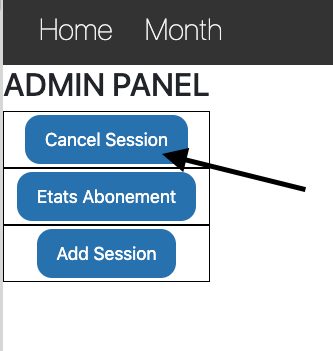
\includegraphics[width=0.4\textwidth,center]{Figures/us9-1}
	\caption{Bouton de navigation de l'administrateur}
\end{figure}

\vspace{\baselineskip}
\begin{figure}[h]
	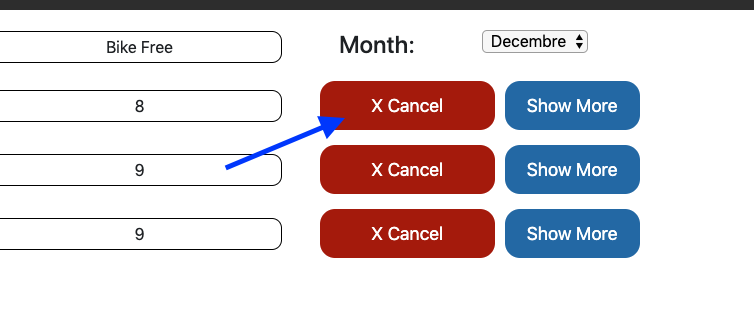
\includegraphics[width=0.8\textwidth,center]{Figures/us9-2}
	\caption{Bouton d'annulation de la session}
\end{figure}


\vspace{\baselineskip}
\subsubsection{Script concernés}
	\begin{itemize}
		\item \Href{https://github.com/victorsmits/Aquabike/blob/master/backend/src/Controller/SessionAdministrationController.php}{SessionAdministrationController.php}
		\item \Href{https://github.com/victorsmits/Aquabike/blob/master/backend/templates/registration/SessionAdmin.html.twig}{SessionAdmin.html.twig}
		\item \Href{https://github.com/victorsmits/Aquabike/blob/master/backend/src/Entity/Session.php}{Session.php}
	\end{itemize}
